\subsection{Intersymbol Interference}

\begin{equation}
    \label{eqn:expl-0}
    R_y[m] = E[(\sum_{k}a_kh[i+m-k]+w[i+m])(\sum_j a_j^* h_j^*[i-j]+w[i])]
\end{equation}

\begin{equation}
    \label{eqn:expl-1}
    E[a_k a_j^*] =
    \begin{dcases}
        E_a \quad j=k \\
        0 \quad j \neq k
    \end{dcases}
\end{equation}

\begin{equation}
    \label{eqn:expl-2}
    E[a_k w^*[j]] = 0
\end{equation}

\begin{equation}
    \label{eqn:expl-3}
    E[w[j]w^*[k]] =
    \begin{dcases}
        \sigma_w^2 = \frac{N_0}{2} \quad j=k \\
        0 \quad j \neq k
    \end{dcases}
\end{equation}

\begin{equation}
    \label{eqn:expl-4}
    \therefore R_y[m] = \sum_k E_a h[i+m-k]h^*[i-k]+ \frac{N_0}{2}\delta [m]
\end{equation}

Hence,

\begin{equation}
    \label{eqn:expl-5}
    R_y[m] = E_a \sum_j h[m+j]h^*[j] + \frac{N_0}{2} \delta [m]
\end{equation}

\subsection{MMSE Equaliser}

\begin{figure}
    \begin{center}
        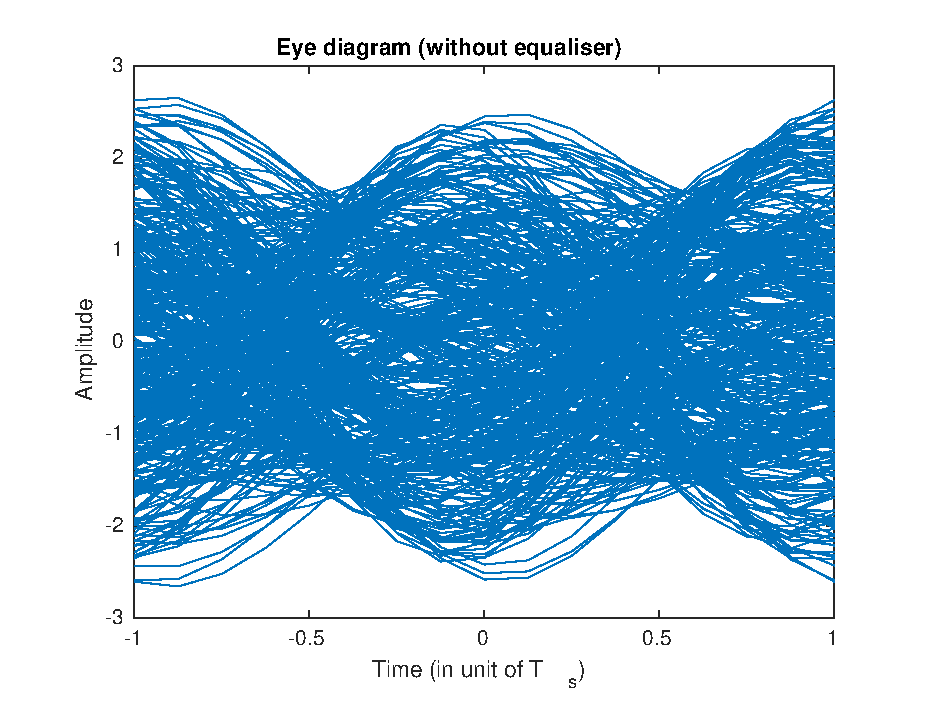
\includegraphics{Equaliser/eye}
    \end{center}
    \caption{}
\end{figure}

\begin{figure}
    \begin{center}
        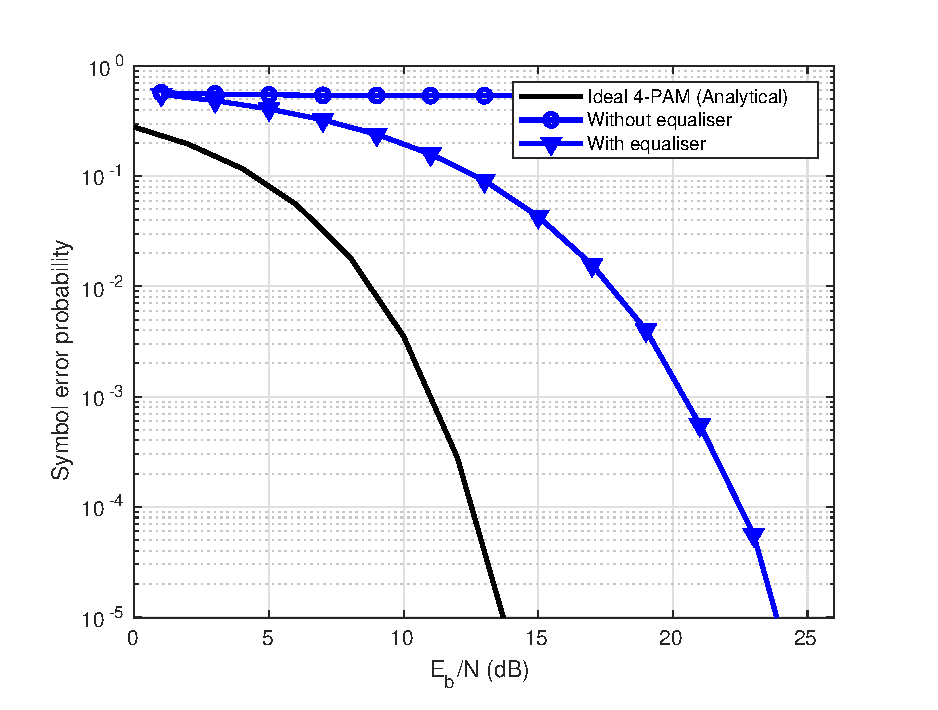
\includegraphics{Equaliser/ber}
    \end{center}
    \caption{}
\end{figure}

\begin{figure}
    \begin{center}
        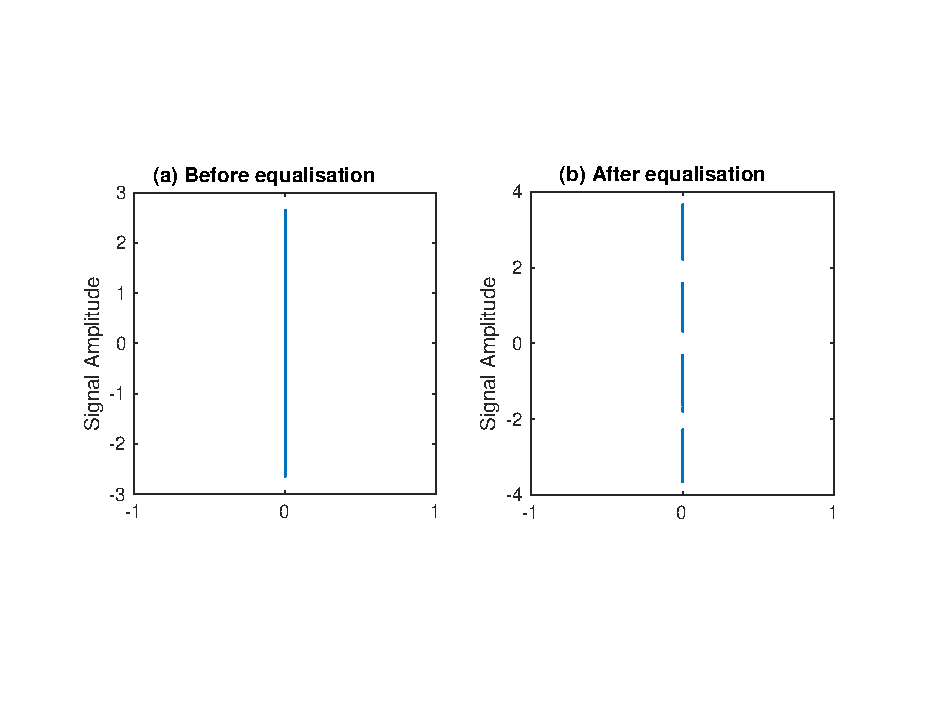
\includegraphics{Equaliser/scatter}
    \end{center}
    \caption{}
\end{figure}

\subsection{Displaying a eye diagram with lab equipment}
